\chapter{Rendre le domicile sensible au contexte}
\begin{preamble}
Ce chapitre présente une approche visant à assurer la fiabilité de la sensibilité au contexte pour les applications d'assistance domiciliaire. 
%de la détection d'activités d'un utilisateur définie par ses interactions avec son environnement. 
Cette approche consiste à rendre explicite un {\em modèle de rôles} joué par les capteurs, à travers des règles, contribuant à assurer que le fonctionnement du capteur correspond à son rôle. Ces {\em règles de conformités} permettent de fournir des instructions détaillées quant à l'installation et le positionnement de capteurs dans le monde physique et assurer la conformité d'un installation déployée par rapport à son modèle durant son exploitation.



% This paper addresses the challenge of making reliable the detection of user activities defined by interactions of user with their environment. This range of context awareness is of the utmost importance for a range of applications supporting daily life activities of a user in their home. Our approach consists of making explicit the {\em model of roles} played by sensors. This model is defined by declaring rules that contribute to ensuring that sensors function in conformance with their expected roles. These {\em conformance rules} take the form of relations that are checked by a Prolog program. This program runs alongside the pervasive computing system; it intercepts sensor readings and continually checks whether they conform to the model of sensor roles, raising an error if they do not.

% We implemented our approach with a complete system combining 1) a pervasive computing platform, 2) sensors and actuators for the home, and 3) a Prolog-based verification layer. This implementation has been applied to the domain of assisted living for older adults. We used deployments made in the home of older adults to validate our tool. Specifically, we demonstrated that our tool can detect a number of anomalies in deployments, ranging from misplacement to obstruction or fall.

% Our approach has many benefits, impacting all the stakeholders of a smart home. Programmers can make their application requirements on sensors explicit as they develop their application, while preventing their code from being polluted with conditional statements. This achieves a  {\em separation of concerns} that contributes to ease the development of pervasive computing applications. Also, when a sensor is shared among different applications, its declared role can be matched against a new application requirement. Furthermore, the model of sensor roles can be shared with the individual installing the sensors. This could be done by providing them with an appropriate representation for the conformance rules to guide in the placement of the sensors.
\end{preamble}
\chpsummary{Contributions}
{
  Une approche qui améliore la fiabilité des application sensibles au contexte pour la surveillance d'activité.;
  Un concept de {\em modèle de rôles de capteurs} est introduit pour capturer les besoins des applications en terme de capteurs, et est vérifié en continu en parallèle de l'exécution des applications.;
  Ce modèle de capteur peut être {\em factorisé} entre les applications, {\em partagé} entre les intervenants, et {\em utilisé} pour les évolutions de la plate-forme.
}
% \newpage
Les applications reposant sur l'informatique ubiquitaire sont profondément liées à la reconnaissance d'activités des utilisateurs. 
La sensibilité au contexte devient alors une clé essentielle pour que ces applications soient acceptées par les utilisateurs.
Par exemple, dans un domicile équipé d'informatique ubiquitaire, la sensibilité au contexte permet à une application de notifier l'utilisateur à propos d'une activité~\cite{CHAN-REVIEW-COMPUTER2008}, {\em uniquement} si l'activité à été oubliée; elle permet de déclencher une alerte pour une porte restée ouverte {\em uniquement} si il n'y a personne dans la zone; elle permet d'appeler l'utilisateur lorsque la cuisinière est restée allumée, {\em uniquement} si elle n'est pas surveillée depuis un certain temps.
Pour intégrer la vie quotidienne de l'utilisateur, il est indispensable que l'application sensible au contexte soit fiable. 
Il est essentiel de minimiser les faux positifs dans la détection de situations nécessitant l'attention de l'utilisateur. Ces notifications issues de reconnaissance de contexte erronés fatiguent l'utilisateur et ralentissent, voire empêchent l'acceptation de la technologie.

La fiabilité d'une application ubiquitaire et sensible au contexte est définie par la fiabilité du système dans son ensemble~\cite{STANKOVIC-OPPORTUNITIES-COMPUTER2005,MENNICKEN-FROM-UBICOMP2014}. En informatique ubiquitaire, le système est principalement constitué d'une couche logicielle et d'une couche matérielle. 
Dans le domaine de l'informatique ubiquitaire, la fiabilité logicielle a été amplement étudiée; des approches à base de simulation ont été proposées~\cite{BRUNO-DIASIM-MOBIQUITOUS2009} pour tester la fiabilité du logiciel avant son déploiement. Ces approches permettent de tester, in-vitro, des scénarios sur des applications, en simulant les interactions de l'utilisateur avec son environnement ({\em e.g.} une ouverture de porte, une présence dans une pièce, la mise en marche d'un appareil). Malgré la rigueur et l'exhaustivité de cette phase de test, la fiabilité logicielle reste dépendante de la fiabilité de la couche matérielle elle-même fournissant les données de contexte.

La fiabilité de la couche matérielle d'un système dépend de nombreux facteurs. D'un point de vue unitaire, la fiabilité relève de celle du capteur. 
Elle peut consister à simplement de vérifier que le capteur fonctionne correctement. Cependant, pour être sensible au contexte, 
une application nécessite les données de plusieurs capteurs~\cite{STANKOVIC-OPPORTUNITIES-COMPUTER2005}. Conceptuellement, un capteur est vu comme jouant un {\em rôle} dans la logique applicative: il mesure les interactions des utilisateurs avec leur environnement. Ainsi, le capteur est supposé être placé de façon appropriée pour mesurer efficacement ces interactions (direction, fréquence, sans interférences, {\em etc.})~\cite{EDWARD-ATHOME-UBICOMP2001}. Quand la caractérisation d'un contexte dépend d'une combinaison d'interactions, le développeur construit un modèle implicite de rôles %qui doivent être 
joués par une combinaison de capteurs~\cite{HENRICKSEN-MODELING-PERVASIVE2002}. Par exemple, un capteur de contact pour la porte d'entrée peut conceptuellement, être couplé avec un capteur de mouvement, couvrant la zone de l'entrée. Une application peut utiliser cette dépendance de capteurs comme suit: si la porte d'entrée est ouverte, mais que la présence de l'utilisateur est détectée à proximité, alors aucune alerte ne doit être envoyée. Si le modèle implicite est transgressé par une défaillance du capteur de mouvement, l'application sensible au contexte est compromise. Il en résulte une notification erronée alertant d'une situation de porte d'entrée ouvert et non surveillée, et ce, même si l'utilisateur est a proximité.

Pour adresser la fiabilité au niveau du capteur, typiquement, le développeur introduit du code pour tester la validité de ce modèle implicite. Cette stratégie consiste à retranscrire des {\em règles implicites} à travers des déclarations conditionnelles réparties à travers le code de l'application. Ces règles contribuent à assurer une lecture des capteurs conforme au modèle implicite. Par Exemple, si une cuisine est équipée d'un capteur de contact sur un placard spécifique et d'un capteur de mouvement, alors, la porte du placard ne doit pas être détectée comme étant ouverte sans une détection préalable d'une présence dans la cuisine. Si cette situation se produit, alors il y a transgression du modèle implicite. De nombreuses raisons peuvent être la cause de cette violation (placement, dysfonctionnement) et conduisent à une intervention pour résoudre le problème. Détecter ces situations est une clé essentielle de la fiabilité des applications d'informatique ubiquitaires sensibles au contexte déployées dans un domicile~\cite{BECKMANN-SOME-UBICOMP2004}.
 

% \subsection*{Contributions}
% This paper makes the following contributions.
% \begin{itemize}
% \item We propose an approach to improving the reliability of context-aware applications dedicated to activity monitoring.
% \item A concept of {\em model of sensor roles} is introduced to capture application requirements concerning sensors,
% and continuously checked alongside running applications.
% \item This model of sensor roles can be {\em factorized} across applications, {\em shared} among stakeholders, and {\em leveraged} for platform evolution.
% \item We present a tool that implements our approach in an assisted living platform.
% \item We validate our tool on real deployments in the home of older adults, demonstrating the effectiveness of our approach.
% \end{itemize}

%\subsection*{Outline}
% The paper is organized as follows. Section~\ref{sec:casestudy} describes a case study used for introducing and illustrating our
% approach. Section~\ref{sec:requirements} analyzes the application needs in terms of sensing abstractions and their
% implicit assumptions about these abstractions. Section~\ref{sec:model} proposes a model for making these assumptions
% explicit and checkable automatically. Section~\ref{sec:architecture} presents the architecture we propose for continuously
% checking the model conformance during execution, or offline. Section~\ref{sec:validation} describes some experimental results validating our approach on data accumulated during an activity monitoring field study. Section~\ref{sec:discussion} further discusses
% some benefits of our approach. Section~\ref{sec:relatedwork} relates our approach to other research works, and Section~\ref{sec:futurework} concludes.


\section{Étude de cas}
Pour illustrer notre approche, nous présentons, comme étude de cas, la surveillance de deux activités de cuisine. Ces exemples sont simples mais complets. Ils utilisent différents types de capteurs pour reconnaître différents types d'interactions entre l'utilisateur et son environnement, dans la cuisine.

La surveillance d'activité est extrêmement dépendante de la population ciblée par les applications d'assistance~\cite{DURICK-DISPELLING-OZCHI2013}. Par exemple, une personne âgée peut simplement avoir besoin d'un rappel pour la réalisation de ses activités quotidiennes~\cite{CAROUX-VERIFICATION-SIGACCESS2014}, alors qu'une population avec des déficiences intellectuelles ({\em e.g.,} syndrome de Down) peut avoir besoin de supervision dans l'exécution d'étapes clés d'une tâche\cite{LUSSIERDESROCHERS-ANALYSIS-DISABILITY2016}.

Pour déterminer {\em quelles} activités doivent être surveillées et {\em comment} elles doivent être surveillées, nous avons besoin d'expertise sur la population ciblée. Des professionnels comme des ergonomes et des ergothérapeutes fournissent cette expertise. Dans notre exemple, un expert définit les activités qui doivent être surveillées dans la cuisine. À partir de cet ensemble d'activités, l'expert détermine {\em quelles interactions} avec l'environnement doivent être détectées pour identifier ces activités. Typiquement, l'expert demande à l'utilisateur de mimer les différentes étapes effectuées pour réaliser une activité~\cite{CAROUX-VERIFICATION-SIGACCESS2014}. Une fois les interactions clés concernant chaque activité intéressante sont identifiées, nous devons déterminer {\em quels capteurs} sont pertinents pour mesurer ces interactions. Cette étape a été étudiée par Beckmann {\em et al.}~\cite{BECKMANN-SOME-UBICOMP2004}. Ils présentent un guide pratique pour installer les capteurs et l'évaluent à travers une étude utilisateurs.

Supposons maintenant que l'expert définit les activités suivantes: (1) la surveillance de la préparation du petit déjeuner, pour envoyer un rappel à l'utilisateur si cette activité a été manquée et (2) la surveillance de la cuisinière pour s'assurer de son utilisation en sécurité.

\subsection{Surveillance de la préparation du petit déjeuner}
Pour surveiller la préparation du petit déjeuner, l'expert du domaine définit des scénarios typiques réalisés par l'utilisateur. 
Un de ces scénarios peut par exemple être décrit ainsi: l'utilisateur (1) fait du café en utilisant une machine à café électrique, (2) prend une tasse depuis un placard spécifique ou le lave-vaisselle, et (3) prend du lait dans son frigidaire. 
À partir de ce scénario, il est possible d'extraire les interactions à mesurer: (1) allumer la machine à café, (2) ouvrir la porte du placard, (3) ouvrir la porte du frigidaire. Pour mesurer ces interactions, un capteur de consommation électrique est associé à la machine à café: si une consommation électrique est captée, alors la machine à café est allumée. Les interactions avec la porte du frigidaire et la porte du placard sont détectées au moyen de capteur de contact. Pour simplifier nous n'avons pas placé de capteur de contact sur le lave-vaisselle, et supposons que dans ce cas, l'action de prendre une tasse ne peut pas être détectée.

\subsection{Sécurité de l'utilisation de la cuisinière}
La sécurité de l'utilisation de la cuisinière dépend principalement de la détection de l'utilisation de la cuisinière et de la présence d'un utilisateur à proximité pour surveiller la cuisson. Un capteur de consommation électrique est utilisé pour détecter si la cuisinière est en fonction, et capteur de mouvement est positionné pour détecter une présence dans un périmètre stratégique autour de la cuisinière (typiquement dans l'ensemble la cuisine).

\subsection{Rendre explicite un modèle implicite}
Pour résumer, les activités à surveiller dans notre cas d'utilisation sollicitent la reconnaissance de cinq interactions avec l'environnement de la cuisine: ouvrir la porte d'un placard spécifique, ouvrir la porte du frigidaire, allumer la machine à café, allumer la cuisinière, et détecter la présence dans la cuisine.

Pour schématiser, dans le contexte de notre cas d'utilisation, la dernière étape de notre méthode consiste à: rendre explicite le modèle implicite qui assure la fiabilité des interactions détectées. Nous savons que chacune des interactions mesurées dans la cuisine doit être précédée par la détection d'une présence. Réciproquement, si une interaction est mesurée sans être précédée par la détection d'une présence dans la cuisine, on peut supposer que les capteurs impliqués ont un dysfonctionnement. Ces règles contribuent à assurer qu'une infrastructure de capteurs fonctionne en conformité avec le modèle de rôles.

\section{Besoins des applications}
Les applications de support d'activité domiciliaire fournissent des services de surveillance et d'assistance pour un utilisateur. Ces services reposent sur un ensemble de données contextuelles relatives à des mesures d'interactions dans l'environnement, comme illustré avec notre cas d'étude.

Cependant, il y a souvent un fossé entre les données brutes, fournies par les capteurs, et le point de vue conceptuel du développeur d'applications sur l'environnement d'interactions. Par exemple, un capteur de contact produit des valeurs booléennes définissant les états ouvert/fermé. Cet état doit être combiné avec l'emplacement spécifique (et/ou un identifiant) du capteur pour rendre l'interaction exploitable par l'application. De plus, plusieurs capteurs combinés, peuvent être requis pour détecter une interaction. Par exemple, la détection d'une présence dans une pièce en forme de L nécessite plusieurs capteurs de mouvements.

\subsection{Rôle}
Du point de vue de l'application, le rôle définit les informations d'interaction directement exploitable par la logique applicative. Ce rôle consiste en un type d'interaction ({\em e.g.,} présence) et l'emplacement de l'interaction ({\em e.g.,}la cuisine). D'un point de vue physique, un rôle définit les besoins qui doivent être satisfaits par un ou plusieurs capteurs pour détecter une certaine interaction. Conceptuellement, les rôles sont positionnés entre la couche physique des capteurs et les applications, comme représenté en Figure~\ref{fig:appreqrole}. Pour être en conformité avec un rôle, les capteurs doivent être disposés correctement en terme de positionnement et de direction. Comme illustré précédemment, détecter une présence dans une cuisine en forme de L nécessite au moins deux détecteurs de mouvements, orientés de façon à couvrir entièrement la cuisine, sans pour autant détecter les mouvements des espaces adjacents ({\em e.g.,} le couloir adjacent à la cuisine). Il est à noter que les rôles permettent la séparation des préoccupations entre les applications et la couche physique des capteurs.

\begin{figure}[!h]
  \centering
  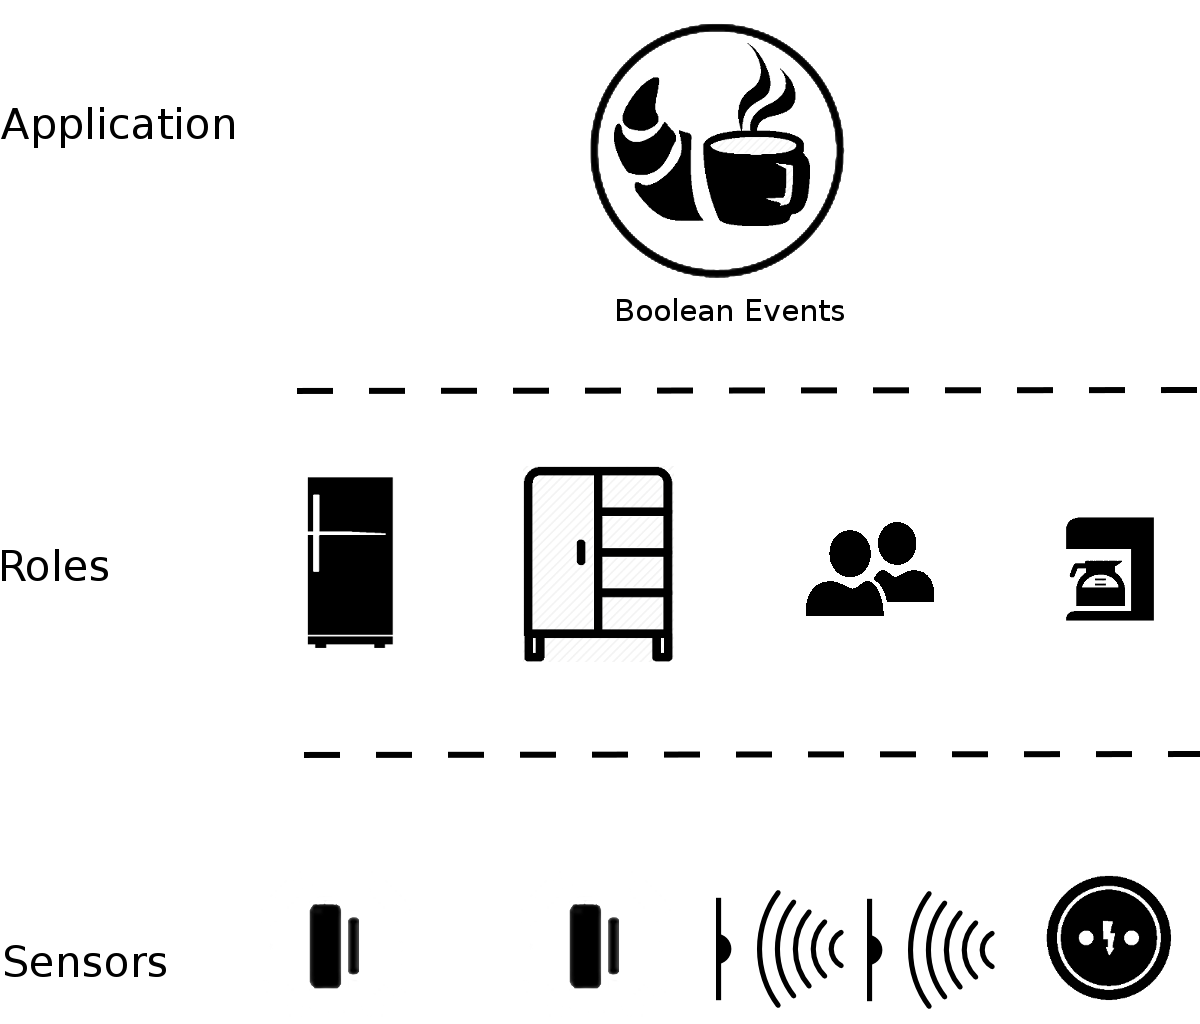
\includegraphics[scale=0.15]{gfx/Roles_etc.png}
  \caption{Application requirements and roles}
  \label{fig:appreqrole}
\end{figure}

\subsection{Sémantiques des rôles}
La sémantique d'un rôle couvre (1) la détection d'une interaction avec l'environnement, produisant une valeur {\em true}, et (2) la détection de la fin de cette interaction, produisant une valeur {\em false}. Ce comportement est illustré dans la Figure~\ref{fig:semofroles}. Un rôle est alors une fonction définie sur le temps et couvrant des valeurs booléennes. Quand une interaction est détectée à un instant, celle-ci produit true, jusqu'à ce qu'elle ne soit plus détectée, alors elle produit false.


\begin{figure}[!h]
  \centering
      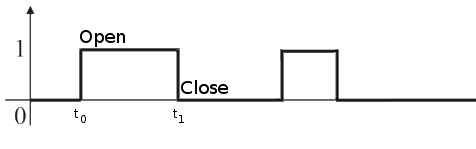
\includegraphics[scale=0.3]{gfx/graph.png}
      \caption{Sémantique des rôles}
      \label{fig:semofroles}
\end{figure}

En pratique, pour fournir cette sémantique temporelle à l'application, l'implémentation d'un rôle doit être filtrée pour isoler les séquences de donnée atypiques (bruit). Par exemple, pour un rôle joué par un capteur de contact, s'il fournit deux valeurs true (ouverture) consécutives, nous filtrons la seconde.

\section{Modèle d'infrastructure}
Les capteurs installés dans un domicile constituent une infrastructure qui supporte les rôles requis par les applications déployées. 
La bonne implémentation des rôles est critique quant à la fiabilité de la sensibilité au contexte de cette infrastructure. 
Cette fiabilité va au-delà des tests unitaires de chaque rôle.

Pour adresser la fiabilité de l'infrastructure, nous proposons de construire un modèle de cette infrastructure qui peut être vérifié. Ce modèle ne prend pas uniquement en compte les rôles individuels, mais également leur conformité par rapport à des règles globales en rapport avec l'infrastructure de capteurs.


\subsection{Les évènements de rôle}\label{archi:algebra} 
La première étape pour expliciter le modèle d'infrastructure en tant qu'ensemble de règle, est de délimiter le domaine des objets sur lesquels les règles pourront agir: les évènements de rôle. Un rôle se compose de trois éléments: (1) une interaction qui s'est produite (2) à une localisation donnée, (3) pendant une période de temps spécifique. Tout d'abord examinons la notion de période. Elle est définie en tant qu'intervalle délimitée par deux horodatage. Tel que, \begin{displaymath}\label{archi:algebra:period1}
 \begin{array}{c} 
  Period = \mathds{N}^2\\
    For~p \in Period, p = <t_1, t_2>~and~t_1~<~t_2
 \end{array}
\end{displaymath}

Une période peut également être vue comme une valeur de temps, de $t_1$ à $t_2$, croissante, qui incrémente d'une seconde -- une granularité plus fine n'est pas nécessaire en pratique. Nous pouvons alors utiliser les opérations basiques sur les ensembles pour opérer les périodes, comme $\subseteq, \supseteq$.

Enfin, un évènement de rôle est une interaction qui est arrivée pendant une période. L'ensemble d'interactions est définie par $Inter$ ({\em e.g.,} Présence, Ouverture, Utilisation). Un ensemble de localisations, $Loc$, spécifie l'emplacement d'intérêt dans le domicile ({\em e.g.,} Cuisine, Salle de bain, Chambre). Les évènements de rôle sont donc définies comme suit.

\begin{displaymath}\label{archi:algebra:event}
  \begin{array}{c}
    e~\in~Event = Inter \times Loc \times Period \\
  \end{array}
\end{displaymath}

Comme l'infrastructure de capteurs surveille le domicile, elle produite des logs de données structurés en flux d'évènements de rôles, définie précédemment. Le log d'évènements de rôles est définie ainsi $log~\in~Log = \mathscr{P}(Event)$

\subsection{Formuler des règles}
Maintenant que les logs d'évènements de rôles sont définies et peuvent ainsi être manipulés, nous nous intéressons aux règles du modèle d'infrastructure. Ces règles sont exprimées en tant qu'ensemble de formules logiques dans le calcul de prédicats du premier ordre. Nous introduisons ces règles en examinant trois exemples de notre cas d'utilisation.

\myparagraph{Présence dans la cuisine.} Cette règle rend explicite la dépendance des capteurs dans la cuisine. En substance, nous voulons exprimer le fait que chaque interaction détectée, qui n'est pas un mouvement, doit être encadré par une interaction de mouvement. Ce faisant, nous exprimons le fait que le capteur de mouvement dans la cuisine entoure toutes les autres interactions dans la cuisine ({\em e.g.,} porte de placard, machine à café). Une fois exprimée, cette sémantique assure la conformité des relevés de capteurs dans la cuisine.

Notre règle de présence dans la cuisine prend un évènement de rôle situé dans la cuisine et un log; définie ainsi. \begin{displaymath}\label{archi:algebra:example}
  \begin{array}{c}
    \forall~<i, Kitchen, p>~\in~Log, i \neq Presence~ \Rightarrow \\
    ~~~~\exists~ <Presence, Kitchen, p'>~\in~Log,~p \subseteq p' 
  \end{array}
\end{displaymath}

\myparagraph{Portes restées ouverte.} Nous supposons que dans un but d'assistance domiciliaire, une porte équipée d'un capteur de contact ne doit pas resté ouvert au-delà d'une certaine période, notée $MAX$. Une telle règle s'applique typiquement sur la porte du frigidaire et sur la porte d'entrée parce qu'elle ne doivent pas restées ouvertes trop longtemps. La durée $MAX$ peut variée en fonction des préférences de l'utilisateur et du type de porte.

Cette règle prend un évènement de rôle d'ouverture et une log; définie ainsi.
\begin{displaymath}\label{archi:algebra:example2}
  \begin{array}{c}
    \forall~<Opening, l, p>~\in~Log \Rightarrow  \# p < MAX
  \end{array}
\end{displaymath}

Notons qu'une porte restée ouverte peut être associée à un dysfonctionnement du capteur, ou bien l'utilisateur a tout simplement oublié cette porte et celle-ci n'est pas surveillée par une application déclanchant une notification de sécurité. Par exemple, la porte du placard de notre cas d'utilisation est surveillée pour rappeler à l'utilisateur de préparer ses repas, non pas pour lui rappeler qu'elle est restée ouverte.

\myparagraph{Non omniprésence.}Certaine règle de conformité peuvent être spécifiques à la localisation d'action de l'application. Par exemple, nos recherches en informatique ubiquitaire est principalement concentrée sur le maintien à domicile de personnes âgées vivant seule. Cette situation nous permet de définir la règle de conformité suivante: un rôle de présence ne peut pas être détecté simultanément à deux emplacements différents. La règle de non onmiprésence est définie ainsi. 
\begin{displaymath}\label{archi:algebra:example3}
  \begin{array}{c}
    \forall~<Presence, l, p>~\in~Log \Rightarrow \\
     ~~~~\nexists~ <Presence, l', p'>~\in~Log,~l \neq l' \wedge ~p' \cap p \neq \emptyset
  \end{array}
\end{displaymath}

En pratique, définir des règles de conformités fournis des instructions détaillées pour installer et positionner les capteurs dans le monde physique. Par exemple, la règle de présence dans la cuisine nécessite que la présence soit reconnue dans la cuisine entière. Une fois un domicile installé, les règles assurent la conformité entre l'installation et le modèle.
%\section{Architecture}
\section{Validation}



Premièrement, nous présentons succinctement l'architecture et son implémentation pour vérifier en continue qu'une installation est conforme à son modèle. Ensuite nous présentons brièvement l'expérimentation que nous avons utilisé pour collecter des données de logs écologiques. Nous définissons ensuite les règles de conformité pour un modèle de rôle dédié à l'assistance domiciliaire pour personnes âgées. Finalement, nous appliquons ces règles sur les logs pour assurer leur capacité à détecter les violations de conformité.

\subsection{Architecture}
Globalement, notre architecture consiste à abstraire les lectures brutes de catpeurs à travers une couche de rôle, alimentant à la fois les applications avec des valeurs haut niveau, et les logs d'évènements de rôle utilisés par les règles de conformités du modèle d'infrastructure. Cette architecture est décrite en Figure~\ref{fig:archi}.

Les évènements de rôles sont traités simultanément par les applications et le composant de log. Ce faisant, la conformité des règles peut etre executée à la volée pour relever les érreurs quand elles apparaissent. Alternativement, les règles peuvent être exécutées hors ligne pour diagnostiquer des problèmes quand un opérateur est disponible pour de la maintenance.

\begin{figure}[!h]
  %\vspace{-0.2cm}
  \centering
  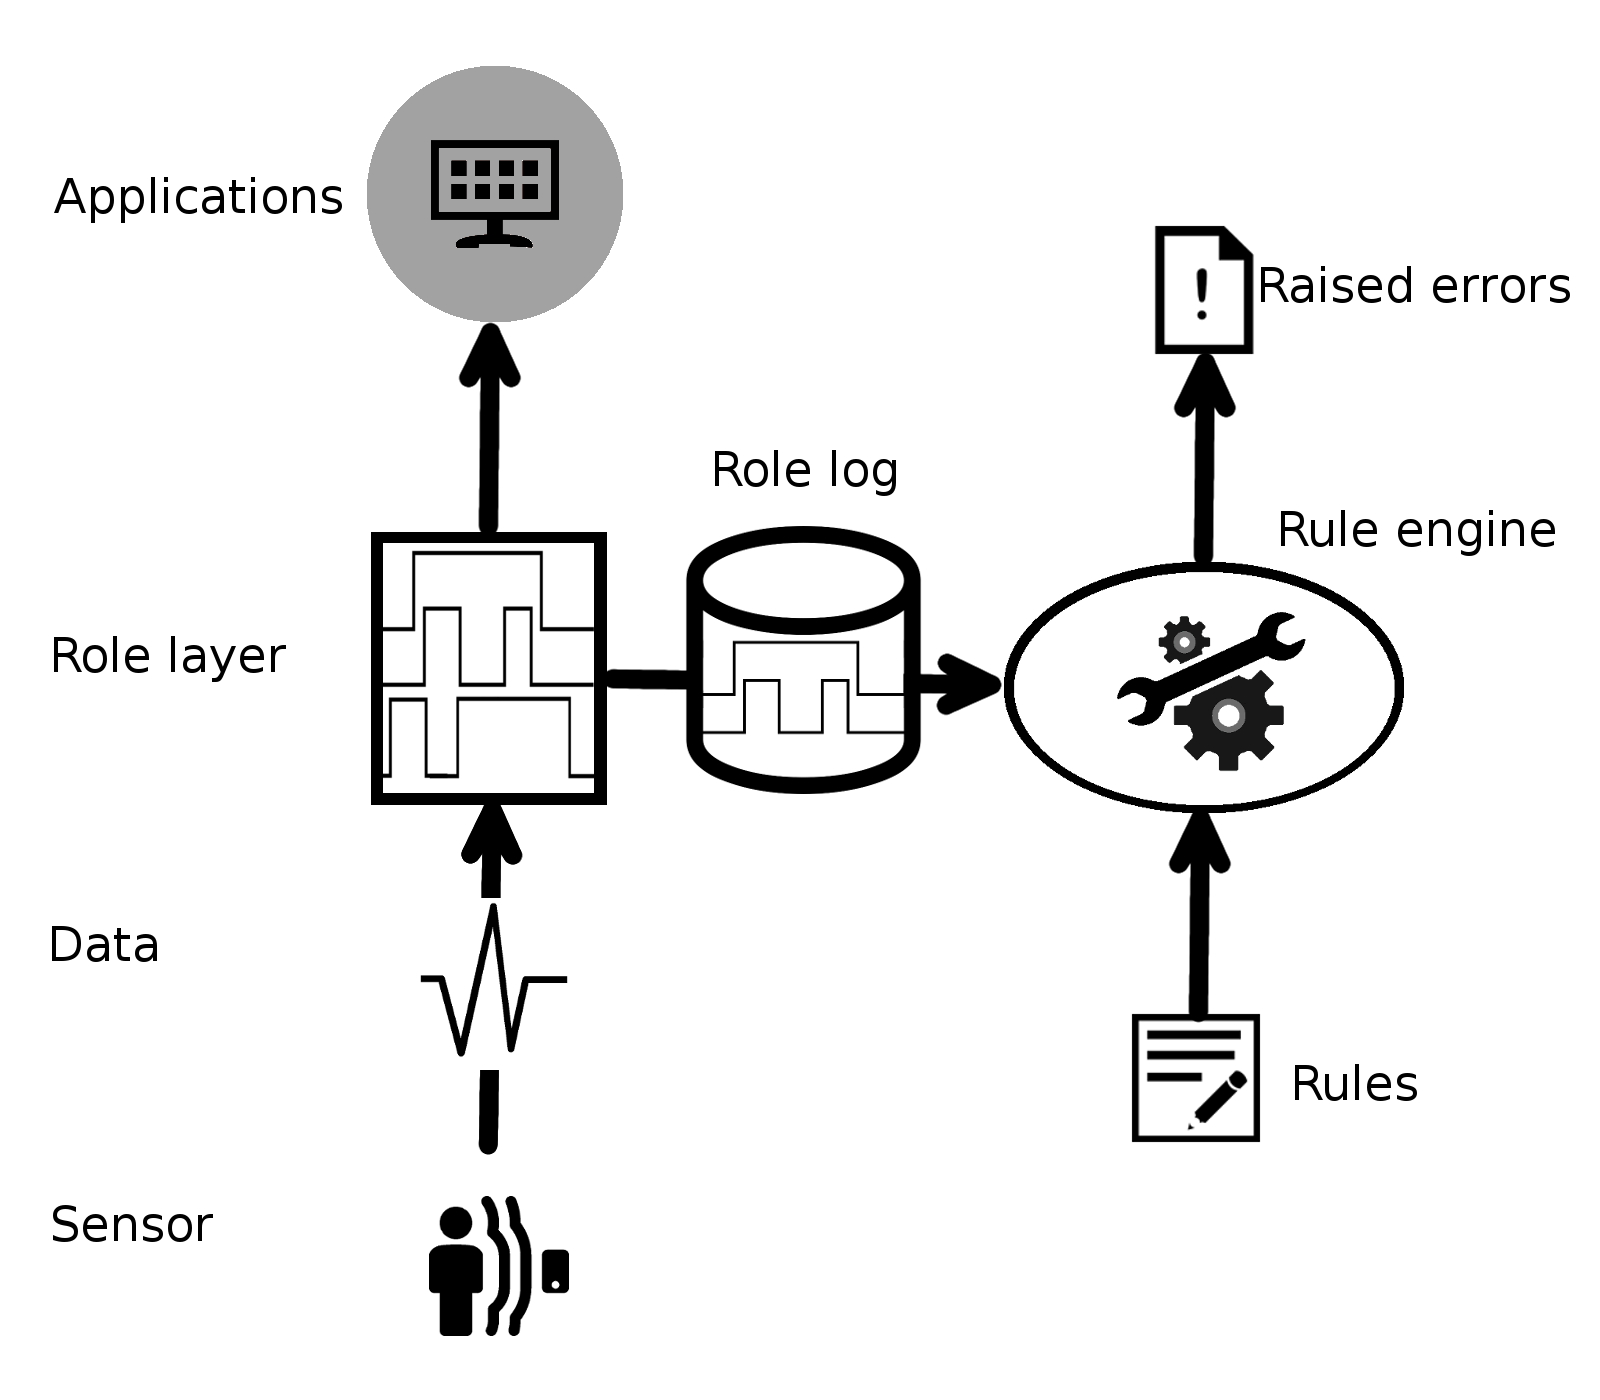
\includegraphics[scale=0.15]{gfx/architecture.png}
  \caption{Architecture}
  \label{fig:archi}
\end{figure}

Au-delà de la maintenance, les logs d'évènements de rôle peuvent aussi être précieux à des fins d'analyse sur l'évolution des activité quotidiennes des personnes âgées. En effet, ces logs permettent des analyses longitudinales qui peuvent, le cas échéant, révéler des dégradation cognitives dues au vieillissement. Ces analyse permettent au professionnel d'adapter l'assistance en supprimant ou installant de nouvelles application pour satisfaire l'évolution des besoins des utilisateurs. 

Également, en faisant levier sur les logs d'évènements de rôle, la reconnaissance d'activités du quotidien peut être ajustée. Par exemple, le seuil de déclanchement des notifications peut être modifié pour prévenir la fatigue de l'utilisateur. De plus, ces logs peuvent servir pour rejouer des séquences d'interactions et déboguer des applications au comportement erroné.


%\subsection{Implementation}\label{algebra:impl}
%This section focuses on the components needed to implement the conformance rules. Our implementation revolves around Prolog because it allows to naturally express our rules and efficiently performs conformance checking.

\myparagraph{Règles.}
Les règles de conformité sont implémenté en tant que prédicats Prolog, de même pour les opérateurs manipulant les évènements de rôles. 
%More precisely, {\em inter\_e/2}, {\em locat\_e/2}, and {\em period\_e/2} allow to access the interaction, the location, and the period of an event, respectively, or to check their equality to a given constant. Operator {\em subset\_e/2} checks whether the period of an event is included in the period of another event.

\myparagraph{Analyser de rôles.}
La plate-forme d'assistance utilisée pour valider notre approche ne fournissant pas la couche d'abstractions nécessaire pour produire les rôle, nous simulons cette couche dans notre implémentation de cette architecture en utilisant un ``analyser de rôles''. Ce composant construit un log d'évènements de rôles en transformant le log de lecture de capteurs les informations associées (type de capteur, localisation, état et horodatage). Cet analyseur de rôle est implanté en un module C++.

\myparagraph{Moteur de règle.}
Ce module traite le log d'évènement de rôle produit par l'analyseur de rôles, et appelle un interpréteur Prolog pour executer chaque règles. De cette façon, quand une règle échoue, le moteur de règle identifie les évènements de rôle impliqué et produit une liste d'évènements de rôles non conformes avec les règles qu'ils ont fait échoués. Ce module est également implanté en C++. 

\subsection{L'expérimentation DomAssist}\label{validation:domassist}
Le projet DomAssist\footnote{ \tiny http://phoenix.inria.fr/research-projects/homeassist} vise à prolonger la vie en indépendance de personnes âgées dans leur propre domicile en leur fournissant une plate-forme d'assistance domiciliaire avec des applications aidant dans les activités du quotidien. Des egrothératpeutes, psychologues et experts en vieillissement ont définie quelles activités sont doivent être surveillées et l'ensemble d'interactions avec l'environnement qui doivent être mesurées.

Pour ce projet, deux types d'applications ont été définit: (1) des application pour surveiller les activités du quotidien et assister l'utilisateur quand elle n'ont pas été effectuée, et (2) des applications de sécurité pour sécuriser le domicile ({\em e.g.,} porte d'entrée restée ouverte). Une étude utilisateur a été conduite en recrutant 24 participants et en déployant à leur domicile notre plate-forme d'assistance domiciliaire pour une durée de neuf mois. Nous avons utilisé les données collectées durant le projet DomAssist pour valider notre modèle d'infrastructure.

\subsection{Modèle}\label{validation:model} 

Les capteurs utilisés dans DomAssist Permettent de mesurer douze points d'interactions avec l'environnement. Les interactions de présence sont mesurées avec des capteurs de mouvement, les ouvertures sont mesurées avec des capteurs de contact, et l'utilisation des appareils électriques est mesurée avec des capteurs de consommation électrique. La configuration de DomAssist en terme de capteurs et leur rôles associés est résumé dans le tableau~\ref{tab:domassist:role}.

\begin{table}[h!]
  \centering
  \begin{tabular}{|l|l|l|}
    \hline
    Room & Role & Sensor \\
    \hline
    \multirow{5}{*}{Kitchen} & Coffee maker in use & EM \\
    & Cabinet door open & CS \\
    & Fridge door open & CS \\
    & Microwave in use & EM \\
    & Presence & CS \\
    \hline
    \multirow{2}{*}{Entrance} & Door open & CS \\
    & Presence & MD \\
    \hline
    \multirow{2}{*}{Bathroom} & Shower in use & MD \\
    & Presence & MD \\
    \hline
    \multirow{2}{*}{Bedroom} & Dressing open & CS \\
    & Bedside lamp in use & EM \\
    & Presence & MD\\
    \hline
  \end{tabular}
\ \\ EM = Electric Meter, CS = Contact Sensor,\\ MD = Motion Detector.
  \caption{Rôles dans DomAssist}
  \label{tab:domassist:role}
\end{table}

Pour des raisons pratiques, notre approche n'a pas été mise en pratique au démarrage du projet DomAssist. Au lieu de quoi, nous avons appliqué notre approche a posteriori. Notre modèle a donc été utilisé rétrospectivement pour vérifier la conformité du domicile de chaque participant en exécutant les règles sur les logs accumulés durant l'expérimentation.

En étudiant l'expérimentation et nos rôles, nous avons spécifier les règles de conformité qui rendent explicite les paramètres de l'étude. C'est à dire, les participants vivent seul (règle de non omniprésence) et des interactions avec l'environnement qui doivent suivre un motif spécifique (porte restée ouverte). D'autres règles ne dépendent pas du but de l'étude et peuvent être généralisées. La règle d'inclusion de présence et ses affinements (intersection de présence et besoin de présence) en sont des illustrations.

Examinons maintenant ces règles.

\myparagraph{Non omniprésence.}
Rappelons que cette règle assure qu'un rôle de présence n'est pas détecté simultanément à deux localisations différentes. En pratique, en fonction de la réactivité des capteurs de mouvements utilisés pour implémenté la détection de présence, quelques chevauchements peuvent survenir et doivent être ignorés. Typiquement, un détecteur de présence signale une absence avec une latence, permettant à l'utilisateur d'être détecté dans une autre pièce. Il peut donc arrivé que la présence soit détectée simultanément dans deux endroits différents pendant un court instant.


% Remove the following rule, as it may be too easily violated by users missing an activity
%\paragraph{Trigger rates}
%We assume that an interaction has to be performed at least once each 24 hours. This element of the model is border closed to activity recognition. A role that has not been recognized for a critical time may be the result of a breach of activity achievement from the user, or a failure from sensors used to measure the interaction. Nevertheless, it is the aim of the activity recognition application to raise user fail. Consequently, in the context of {\HomeAssist} installation, this rule is used to raise failure regardless of user failure.

\myparagraph{Porte restée ouverte.}
Cette règle assure que la période d'un rôle d'ouverte ne dure pas plus d'un certain temps (trois heures dans notre configuration). Notons que cette rèlge est exécutée sur les logs d'évènements de rôle et ne prend pas en compte la façon dont les applications d'assistance peuvent réagir à une telle situation. Par exemple, DomAssist contient une application qui surveille la porte d'entrée et notifie l'utilisateur quand la porte est restée ouverte et sans surveillance, pour quelques minutes (la durée est configurée en fonction du l'utilisateur). En pratique, quand elle est appliquée aux logs de notre études, cette règle détecte dans la plupart des cas des problèmes d'installation. Une des raisons est que les participants sont routinisés dans leur activités~\cite{BERGUA-RESTRICTION-IJAHD2013} et n'ont pas décliné congnitivement de façon significative durant l'étude.

\myparagraph{Inclusion de présence.}
Chaque pièce pour laquelle une interaction doit être détectée est équipé avec un détecteur de mouvement. Par concéquent, nous avons généralisé la règle de présence dans la cuisine comme suit: toute interaction a une localisation donnée, qui n'est pas une présence, doit être inclue dans un rôle de présence à la même localisation. 

% In practice, this rule may fail to apply to a specific location: the entrance. Indeed, when users comes back home, they first open the entrance door, then come inside the home to be detected by the motion sensor. Thus, the Door opening role event cannot be surrounded by the Presence role event because the latter one is measured inside the home.  To resolve this problem, the Presence inclusion rule is not applied to the roles related to the entrance. To refine the diagnostic of the Presence inclusion rule, we introduce next two rules towards identifying the cause of the violation.

\myparagraph{Intersection de présence.}
L'inclusion de présence peut être trop contraignante pour s'appliquer à certaines situations. Parfois, nous devons simplement nous assurer que la présence et d'autres interactions ont une intersections non-nulle quand elle sont située dans la même pièce. Une telle règle s'applique dans l'entrée du domicile, équipée d'un capteur de contact sur la porte d'entrée et un capteur de mouvement pour la zone de l'entrée. En effet, si l'utilisateur ouvre la porte depuis l'extérieur ou l'intérieur, les rôles de présence et d'ouverture ont une période de temps durant laquelle leur intersection est non-nulle.


% Every role event, which is not Presence, must have a non-empty intersection with a Presence role event at the same location. If this rule is also violated, it might be the case that the presence detector is not placed correctly with respect to the non-presence interaction. Alternatively, the presence detector might be completely obstructed. To help distinguishing between these two situations, we defined the following even more lenient rule.

\myparagraph{Besoin de présence.}
Pour s'assurer que le détecteur de mouvement est toujours actif même si il est mal positionné, nous introduisons la règle suivante: chauqe rôle, qui n'est pas une présence, doit être accompagné d'un évènement de rôle présence à la même localisation. Cette présence doit arriver au même moment plus ou moins dix minutes. Cette règle rend explicite le fait que le capteur de mouvement est toujours couplé avec un ou plusieurs autres capteurs dans notre configuration. La violation de cette règle indique principalement que le capteur de mouvement ne fonctionne pas correctement, il est toujours enregistré dans le système, mais n'émet plus aucune donnée.

% In theory, the misbehavior could also be due to a false positive in the non-presence interaction. However, this situation never occurred in our experiment.

% \paragraph{Presence dependency}check if a role event recognition which is not a presence is subset by a presence event recognition at the same location
% \begin{itemize}
% \item Entrance : Presence cannot overlay opening, exception replacing subset by intersect  
% \end{itemize}
% \paragraph{Tolerant presence dependency}replacing subset by intersect for all role not presence
% \paragraph{Presence requirement} for each role not presence, check if a presence is recognized at any time at the same room
% \paragraph{Trigger rates}check if a role is recognized at least once in 24 hours
% \paragraph{Long period}check if a role period lasts less than 3 hours
% \paragraph{Teleportation}check if a presence event recognition is not intersect by a presence event in another location
% \begin{itemize}
% \item due to timeout of motion detector used, needs to set intersect tolerance with sensor timeout value
% \end{itemize}

\subsection{Méthodologie}\label{validation:methodology}
Nous avons collecté les logs de données des habitations de 24 participants, âgés de 80 en moyenne et habitants seuls. Les données collectées couvrent une période de neuf mois. Cependant, des problèmes techniques ({\em e.g.,} Accès internet, passerelle de capteurs, serveur) nous ont poussé à ignorer certaines périodes de temps; ces problèmes peuvent être directement détectés au niveau de la plate-forme. Les logs de DomAssist ont également été nettoyés en éliminant les évènements de rôle non conformes. Ces derniers peuvent être détectés par un simple système de surveillance de heartbeat.
% Indeed, every sensor emits a heartbeat signal, whose absence is automatically detected by the lower layers of the platform and signalled as a sensor failure.

Nous avons le plan de chaque domicile des participant ainsi que le positionnement des capteurs. Cette information est utilisée pour diagnostiquer les problèmes quand des violations de conformités arrivent dans les logs. D'autres ressources utilisées pour diagnostiquer les violations ont été utilisées comme les fichiers de suivis des interventions remplis par les professionnels chargés de faire passer des questionnaires à chaque participants durant la durée de l'étude.


% \item Utilisation des plans des installations pour comparer les erreurs relevee par les regles au placement des capteurs (Permanent non-conformance) 
% \item Utilisation du fichier du suivit des visites pour verifier si les regles relevent les memes problemes (Emerging non-conformance) 
% \item Comparaison des différents patterns de resultats de regles pour les erreurs relevee dans les plans ou durant l'experimentation pour identifier des defaillances qui n'auraient pas \'et\'e relevee

\subsection{Résultats expérimentaux}\label{validation:results}


%Our goal in pruning the logs of HomeAssist was to show that our approach could detect anomalies, beyond what simple fault tolerant mechanisms could do. 

Le modèle définit pour DomAssist permet de lever deux types d'anomalies: 1) {\em les non-conformités permanentes} réfèrent à une règle systématiquement violée, indiquant des non-concordances permanentes entre l'infrastructure et le modèle; 2) {\em les non-conformités émergentes} correspondent a une règle qui est vérifié la plupart du temps, mais échoue occasionnellement. Examinons quelques instances de ces anomalies.

\myparagraph{Non-conformités permanentes}
Dans un domicile, l'interaction d'ouverture est détectée pour la porte de placard de la cuisine mais les règles inclusion de présence et intersection de présence échouent systématiquement. Cependant, la règle de besoin de présence n'échoue jamais, indiquant que la porte de placard est ouverte mais jamais entourée par une interaction  de présence dans la cuisine; la présence est détectée à des moments sans rapport. La consultation des documents relatifs à cette installation ont montré que ce placard n'est pas localisé dans la cuisine mais dans une pièce attenante, comme montré en Figure~\ref{fig:map}. Cette situation montre un problème dans la définition du modèle pour cette installation. En conséquence, nous avons réparé le modèle de cette installation en y supprimant les règles inclusion de présence et intersection de présence.

Dans ce même domicile, un autre problème à été identifié: la règle inclusion de présence échoue systématiquement sur le rôle d'ouverture du frigidaire, mais l'intersection de présence n'échoue jamais. Même si le frigidaire est localisé dans la cuisine, le capteur de mouvement utilisé pour mesuré la présence dans la cuisine, n'a pas été positionné pour couvrir l'ensemble de la cuisine, comme montré en Figure~\ref{fig:map}. Ce problème provient dans ce cas d'une erreur à l'installation et sa réparation requière simplement de changer le positionnement du capteur de mouvement. %However, because we retrofitted HomeAssist in our work, this operation could not be done.

Nous avons observé la même situation dans deux autres domiciles pour lesquels le placard de la cuisine équipé d'un capteur de contact est en fait situé en dehors de la cuisine.

Généralement, ces problèmes surviennent quand la plate-forme d'assistance est déployée à large échelle. Dans ce contexte, les installations sont faites par un professionnel et non par les chercheurs qui ont conçu la plate-forme et donc possèdent un savoir implicite sur la bonne manière de déployer. Dans notre cas, même pour 24 domiciles, quelques installations ont été faites par des membres n'ayant pas ce savoir et ont manqué certaines règles implicite.

\begin{figure}[!h]
  %\vspace{-0.2cm}
  \centering
      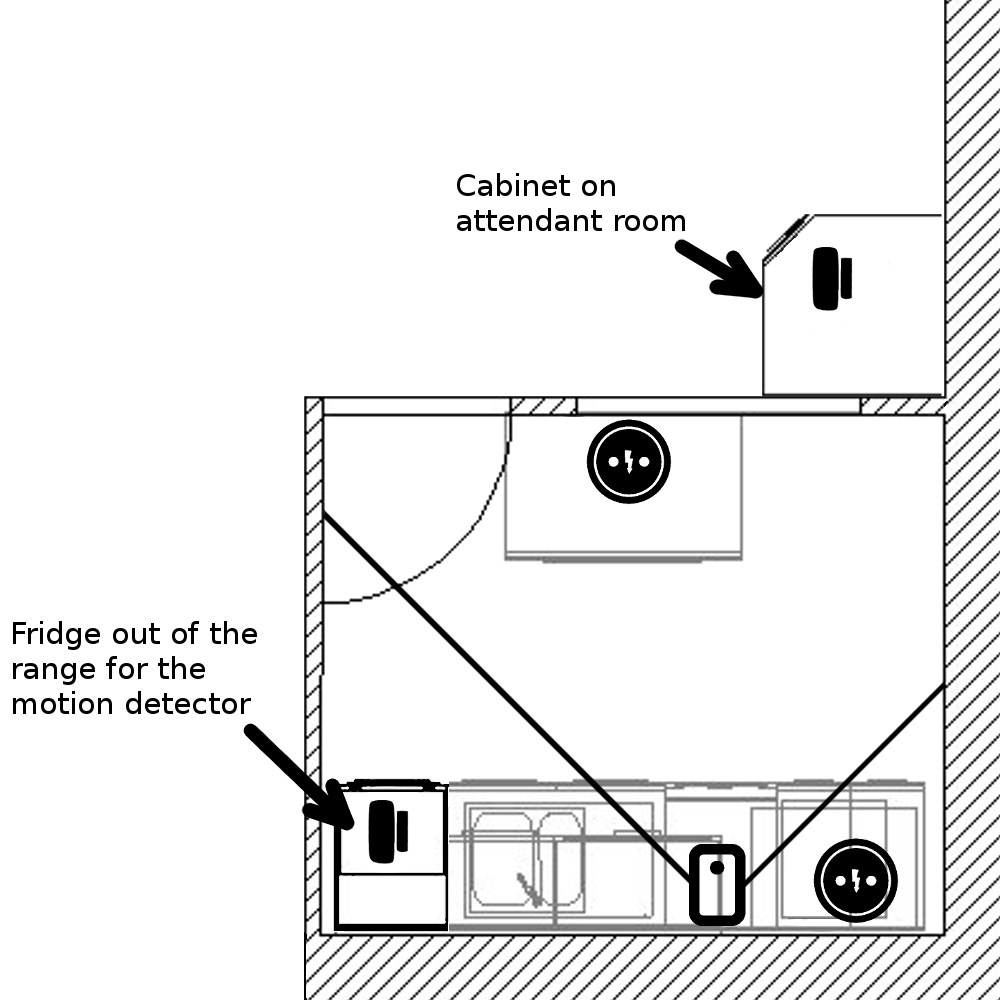
\includegraphics[scale=0.2]{gfx/map.png}
      \caption{Installation issues}
      \label{fig:map}
\end{figure}

Si notre outil avait été utilisé dès la phase de déploiement, il aurait été possible de détecter les anomalies d'installation dès le départ, pendant l'installation ou dans les premiers jours d'exploitation. Parallèlement, une fois déployés, des règles supplémentaires peuvent affiner les modèle pour prendre en compte des spécifications imprévues ({\em e.g.,} cuisine en forme de L). Une fois l'installation ou le modèle réparé, le modèle aide à la détection d'anomalies qui ne sont pas arrivées au moment de l'installation, mais après une période de fonctionnement normal.

\myparagraph{Non-conformités émergentes.}
Un motif de non-concordance a été observé dans cinq domiciles à différentes périodes de temps. Pendant plusieurs jours, la règle inclusion de présence à été violée par une absence de présence dans la cuisine causée par un capteur de mouvement qui dysfonctionne. Dans chacun des cas, les règles d'intersection et de besoin de présence étaient également violées durant ces périodes. Cette dernière règle montre qu'aucun rôle de présence n'a été reconnu durant les 20 minutes entourant cette violation. Les résultats de ces règles fournissent de précieuses informations pour trouver la cause des dysfonctionnement relevés. Il est alors raisonnable de supposer que la cause de cet échec de la règles et un dysfonctionnement temporaire du rôle de présence. Cela suppose que le capteur de mouvement a put être obstrué ou mal orienté. 

Une situation similaire est arrivé dans l'entrée de deux autres domicile: la porte était ouverte mais aucune présence n'a été détectée.

La porte restée ouverte a été observé dans quatre domiciles à différents endroits comme le frigidaire, le placard de la cuisine ou la penderie ({\em i.e.,} la porte est restée ouverte plus de trois heures). D'après les fichiers de suivi des interventions de DomAssist, les utilisateurs concernés ont été questionnés après quelques jours sur les comportements erronés des applications reposant sur ces interactions. Ils ont indiqué que les capteurs de contact étaient tombé. Les installations ont alors été réparée par les techniciens chargés des interventions. Notre modèle, si il avait été disponible durant cette expérimentation aurait permis de rapporter ces incidents, et de les réparer plus rapidement. Cette réactivité est une clé pour les application sensibles au contexte. Elle fait la différence entre une application utile, et une application qui harcèle l'utilisateur avec des notification non pertinente.

\section{Discussion}\label{sec:discussion}
Un modèle explicite d'une infrastructure est capable de détecter les dysfonctionnements du systèmes durant la phase d'installation ou pendant l'exploitation normale. Comme suggéré par certains de nos exemples, une fois une erreur détectée, quelques techniques de diagnostique peuvent être utilisés pour identifier les rôles qui sont la source de l'erreur.  

Premièrement, si plusieurs règles sont violées en même temps, et que ces règles concernent des ensembles de capteurs qui se chevauchent, il est alors probable que le rôle à la source de cette erreur soit à rechercher à l'intersection de ces ensembles. Par exemple, quand la règle intersection de présence échoue en même temps pour le rôle présence dans la cuisine et pour différentes interactions qui ne sont pas des présences (frigidaire, placard, {\em etc.}), on peut en déduire avec une forte probabilité que le rôle défaillant est la présence dans la cuisine. 

Deuxièmement, concevoir une version raffinée d'une règle qui vérifie un ensemble de capteurs ou est un sous-ensemble de la règle de base, peut s'avérer utile pour diriger la recherche d'un rôle défaillant ou d'un capteur qui dysfonctionne. Cette idée est illustrée dans notre modèle pour DomAssist. Il y a une chaîne de trois règles $R_i$ avec des conditions de plus en plus relâchées: inclusion de présence, intersection de présence et besoin de présence. Toutes ces règles sont du type $p \rightarrow q_i$ pour $(i=1..3)$ où le postulat $p$ est identique mais la conclusion $q_i$ est de plus en plus faible. Il y a une implication tout au long de la chaîne, $R_1 \rightarrow R_2 \rightarrow R_3$, ou inversement, quand une des règles échoue, les règles les plus fortes échouent également. Basé sur l'analyse des règles, on peut définir un arbre de décision comme celui en Figure~\ref{fig:bdd} pour aider au diagnostique.

%Secondly, designing refined versions of a given rule that check a set of sensors or subsets of it, may be useful to direct the search of the failing role or malfunctioning sensor. This idea is illustrated in our model for HomeAssist. There is a chain of three rules $R_i$ that increasing relax conditions: presence inclusion, presence intersection, and presence requirement. All these rule are of the type $p \rightarrow q_i$ for $(i=1..3)$ where the premise $p$ is identical but the conclusion $q_i$ is increasingly weaker. Thus, there is an implication relation along the chain, $R_1 \rightarrow R_2 \rightarrow R_3$, or conversely, when one of the rules fails, stronger rules also do. Based on rule analysis, one can derive a binary decision tree such as the one in Figure~\ref{fig:bdd} for helping the diagnosis.

\begin{figure}[!h]
  %\vspace{-0.2cm}
  \centering
      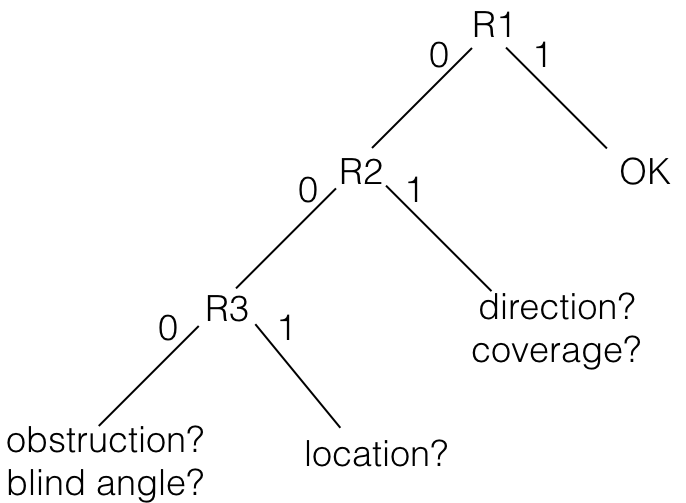
\includegraphics[scale=0.3]{gfx/bdd.png}
      \caption{Binary decision tree for helping the diagnosis}
      \label{fig:bdd}
\end{figure}



%When studying some of the systematic mismatches between the installation and a correct model, one may legitimately ask: How come these installation issues were undetected by conventional tests at installation time? For instance, the fridge or cabinets placed outside the kitchen would have necessarily failed any test of the breakfast monitoring application. This argument is valid: all {\em installed} applications were indeed tested in every home at installation time. However, the experimental protocol allowed participants to choose which applications to activate, based on their needs and preferences. As a result, the breakfast monitoring application was not installed in several homes, hence the undetected installation anomalies. If our model had been used at installation time, the installations could have been certified as conform to the model, validating all applications based on this model.

L'utilité de notre approche pour s'assurer continuellement la conformité d'une infrastructure va au-delà de notre étude. Premièrement, un modèle d'infratrustructure fourni un modèle de référence pour les des applications disponibles dans un catalogue en ligne, comme un Appstore: une application peut être installée du moment qu'elle est conforme au modèle d'infrastructure. Deuxièmement, vérifier le modèle au moment de l'installation réduit les besoins de tests pour {\em toutes} les applications déployées pour une installations donnée, pourvu que le modèle couvre toutes les hypothèses requises par les applications.

\section{Conclusion}\label{sec:futurework}
Nous avons montré que les applications sensibles au contexte produisent fréquemment des suppositions implicites sur l'infrastructure de capteurs. Ces suppositions sont typiquement traduites en déclarations conditionnelles qui polluent le code avec des préoccupations non fonctionnelles. Cette approche défensive peut être évitée en exprimant ces suppositions, non pas dans le code des applications, mais en les factorisant en un modèle explicite d'infrastructure de capteurs. Non seulement la violation d'une telle règle permet d'alerter rapidement sur un dysfonctionnement de l'installation, mais contribue également à diagnostiquer le problème. Une telle approche permet non seulement de s'assurer de la fiabilité de la sensibilité au contexte des applications d'assistance domiciliaire, mais également la définition du modèle, permet de de fournir des instructions détaillée quant à l'installations des capteurs dans le domicile, randant ce dernier sensible au contexte.



% Our approach has been implemented in the context of an assisted living platform, running a set of applications dedicated to assist senior users. Our tool was applied to real sensor data collected during a 9-month field study, consisting of 24 participants aged 80 on average. The results show that some latent installation mistakes could have been found at installation time, using our model. Furthermore, several sensor problems that occurred during operation could have been detected on the fly and repaired more promptly to ensure the reliability of context-awareness applications.

% In future work, we will apply our method in a larger deployment consisting in hundreds of installations. This setting will allow us to quantify in more detail the improved reactivity in detecting emerging infrastructure issues, remotely diagnosing the underlying failure, and repairing the platform on-site. Another future work will consist of proposing log visualisation techniques and tools that contribute to identify new rules for the model by recognizing regular event patterns and anomalies. 